\documentclass[a4paper,11pt]{report}
\usepackage[T1]{fontenc}
\usepackage[utf8]{inputenc}
\usepackage{lmodern}
\usepackage[english]{babel}
\usepackage{amsfonts}
\usepackage{hyperref}
\usepackage{graphicx}
\usepackage{subcaption}

\title{Work report from 12/12/2013 to 03/01/2014}
\author{Rafael Reggiani Manzo}

\begin{document}

\maketitle
\tableofcontents

\begin{abstract}
  This document is intended to make easier for me to explain on what I've been working on, as well as remembering about last meetings and objectives.

  This time I've computed a lot of tensor statistics from which I tried to extract some information.
\end{abstract}

\chapter{Previous meeting}
Here follows a brief recapitulation from our last meeting on 12/12/2013.

  \section{What was presented}
  There I've showed a mean diffusivity (MD) threshold mask that was then clustered to eliminate noises. Given that my objective is to identify crossing regions on a given MRI, you've told me that the MD values isn't the tight one to use for this task.

  \section{Next steps}\label{sec:next-steps}
  Then, you've asked me to create a new threshold mask for fractional anisotropy (FA) values, making sure that I was obtaining the right eigenvalues for that and using the normalized FA equation. With that I'd filter out gray mater regions (FA values lower then 0.2).

  Next to that you've asked me to extract other tensor metrics: radial diffusivity (RD); toroidal curvature (TC); and toroidal volume (TV). Then cluster for each one of those obtaining regions for which I'd calculate for each metric again the mean and standard deviation.

  Finally, apply all that with the high resolution dataset which you've gave me access to.

\chapter{Work done}
Beyond what was discussed previously (\ref{sec:next-steps}), I wasn't feeling that I've read enough yet. So I've decided to search for more references which I'll enter in details right after this (\ref{sec:more-references}).

Another thing that I've worked really hard but I'll not enter in details here was on the quality of the code I've been producing. So I've covered all the code with unit tests and, as I'm writing pure in Python 3.3, I'm also making sure that the style is following pylint\footnote{Pylint is a tool that inspects Python coding errors, pieces of code too complex and style issues like line length. For more information please visit: \url{http://www.pylint.org/}} directives. Finally, since one of the objectives is to process large amounts of data, I've took precaution to take full advantage of CPU multi threading and memoization techniques.

  \section{More references}\label{sec:more-references}
  This was not part of what we've discussed on our last meeting, but I'm still feeling that I haven't read enough yet. So, I've found three new articles that I'd like to discuss:

  \begin{enumerate}
    \item Probabilistic Monte Carlo Based Mapping of Cerebral Connections Utilising Whole-Brain Crossing Fibre Information. Geoff J. M. Parker, Daniel C. Alexander
    \item Diffusion Anisotropy Measurement of Brain White Matter Is Affected by Voxel Size: Underestimation Occurs in Areas with Crossing Fibers. H. Oouchi, K. Yamada, K. Sakai, O. Kizu, T. Kubota, H. Ito, T. Nishimura
    \item Fiber Crossing in Human Brain Depicted with Diffusion Tensor MR Imaging. Mette R. Wiegell, Henrik B. W. Larsson, Van J. Wedeen
  \end{enumerate}

  The number 1 is probably something really similar to what I'm trying to achieve: a pre-mapping of fiber crossing regions to improve tractography's accuracy on that regions. The main difference is the probabilistic approach that it proposes. It's an article from 2003 with lots of spelling errors, so I'm not sure about it's credibility.

  The second and third articles were interesting to bring to my mind some aspects of the problem that I haven't thought about before. The article number two shows the FA values, for some brain regions well known as crossing regions, may vary depending on the voxel dimensions. Finally with the number three I've learned that, besides the cases of simple fiber crossing and fiber kissing, there two other cases that I've not considered yet: fiber spreading; and high curvature fibers.

  \section{Correctness}
  Besides the mentioned unit tests that were made. I've made some visual confirmations that what I've been calculating and the outputs from that algorithms were correct by comparing with the result obtained from Bio Image Suite (MIG's version).

  \begin{figure}[!ht]
    \centering

    \begin{subfigure}[t]{.49\textwidth}
      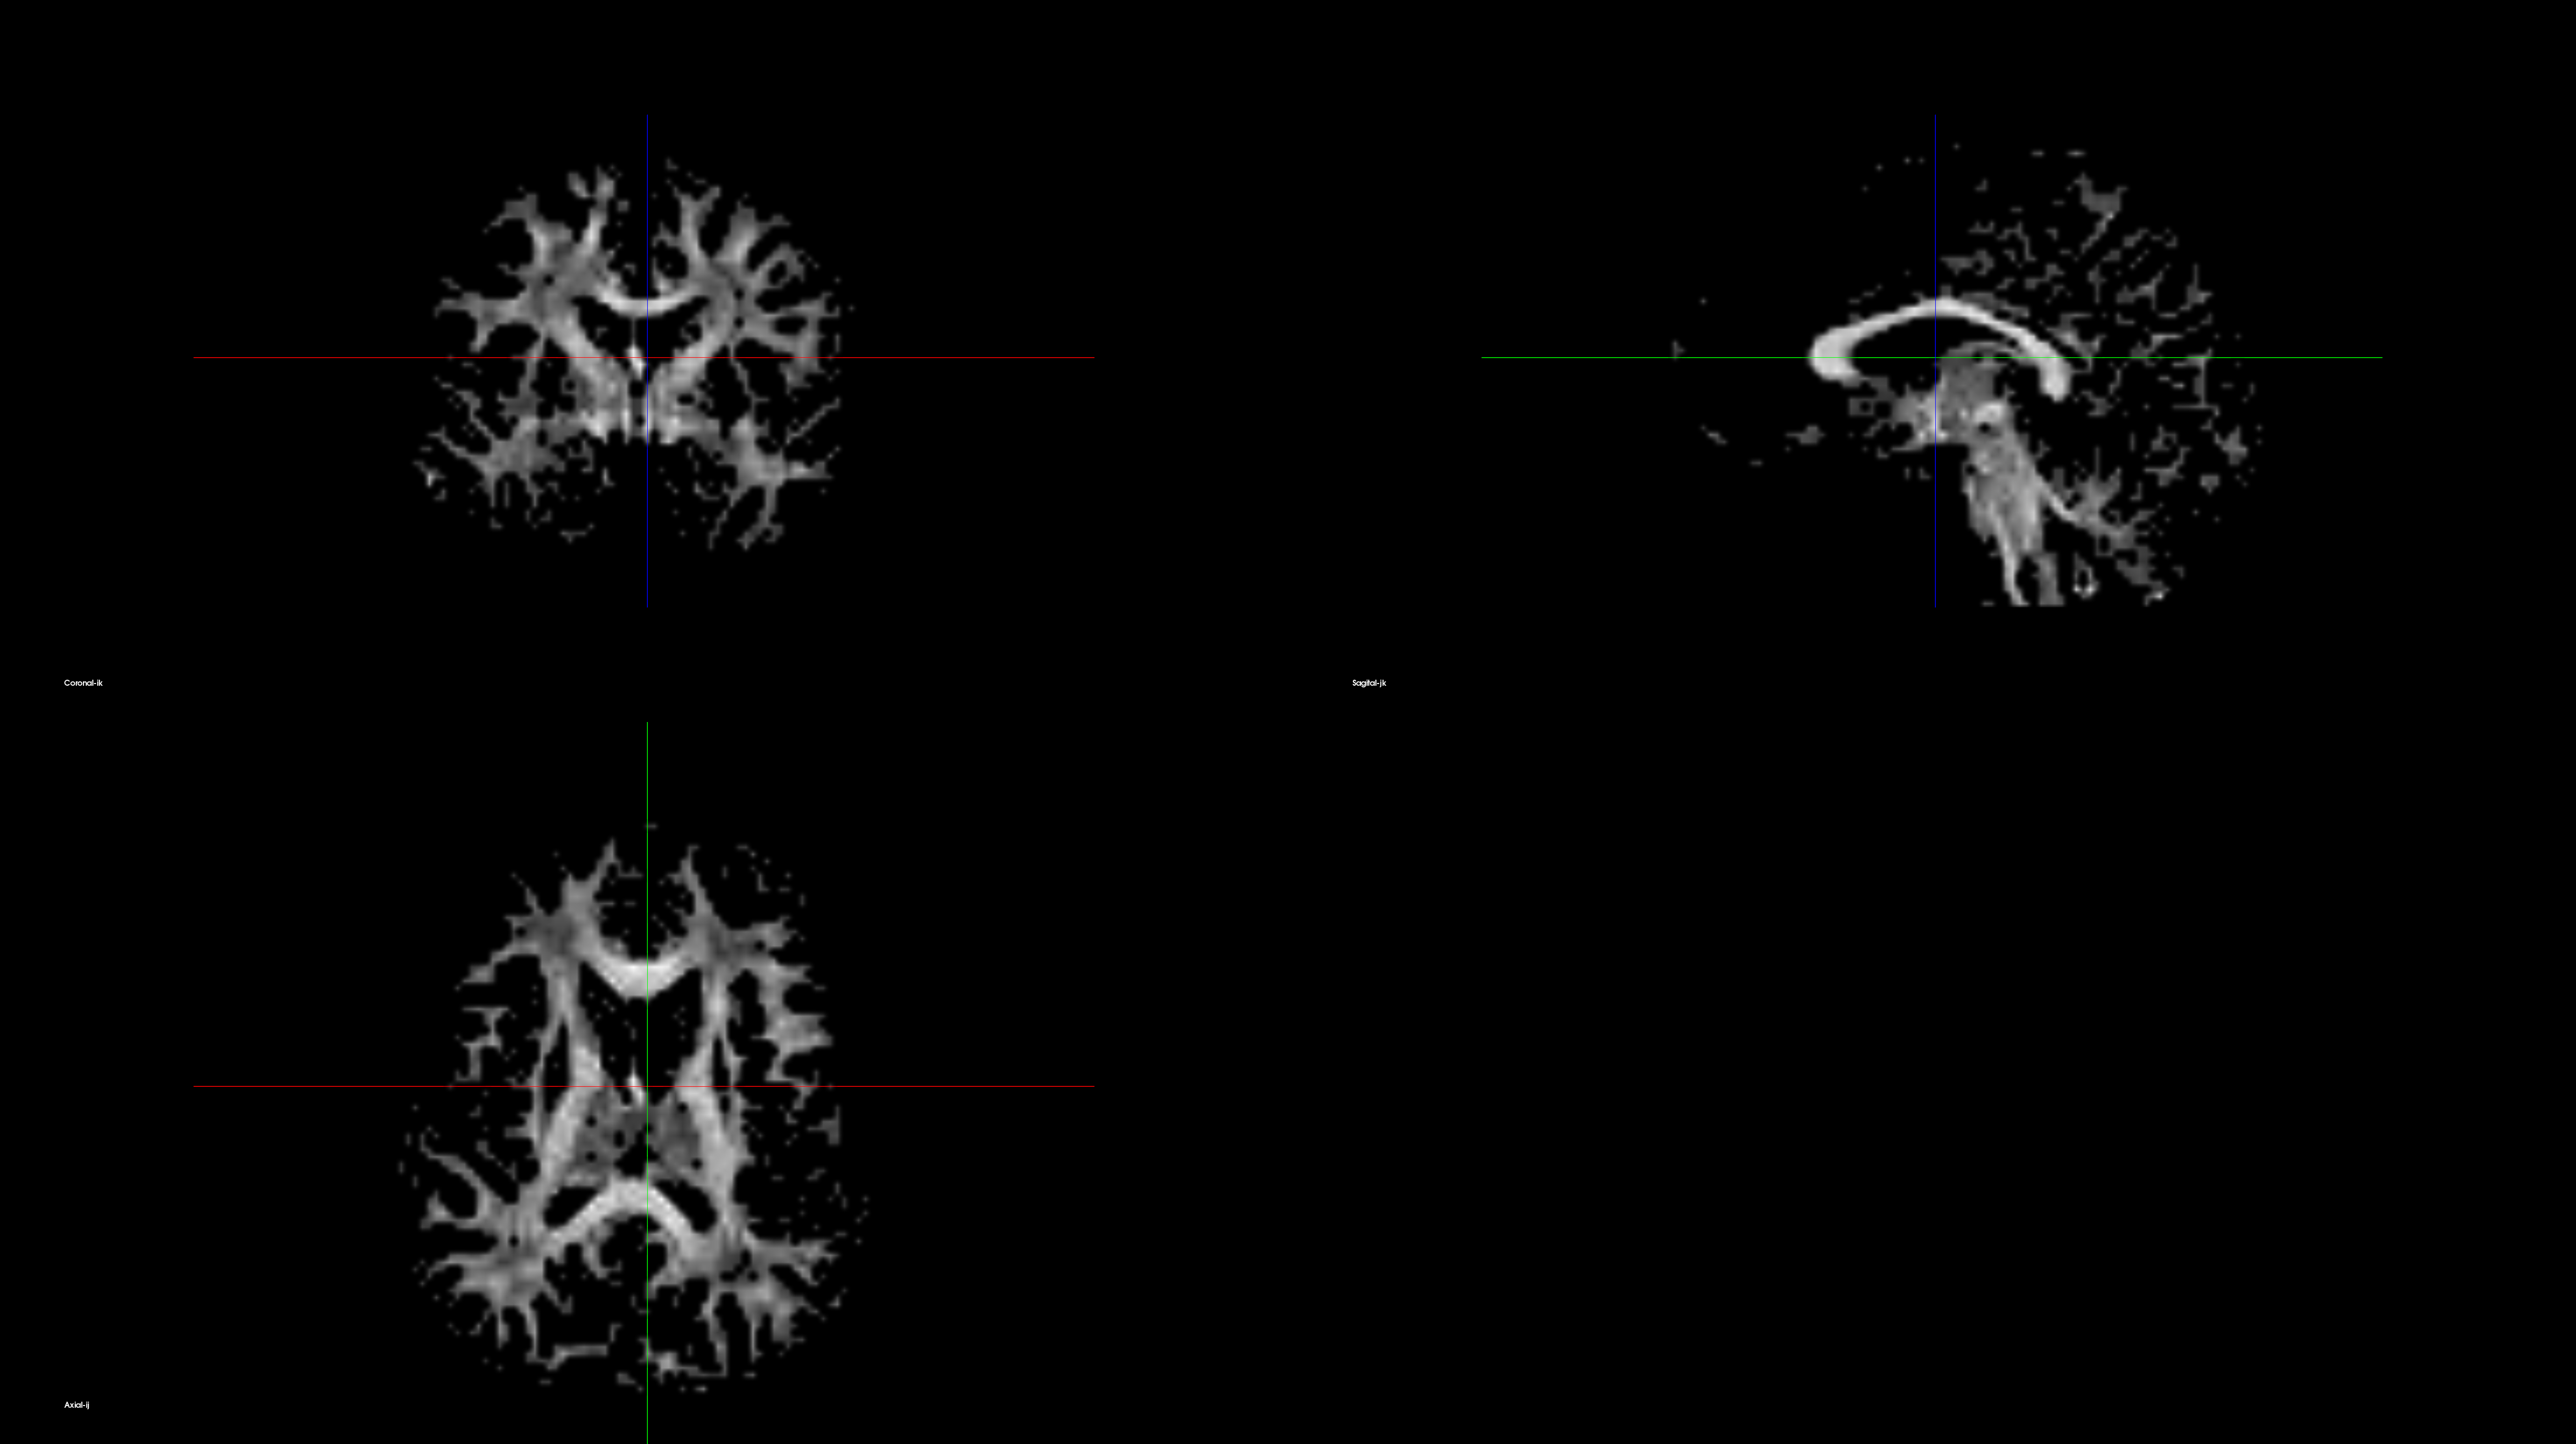
\includegraphics[width=1\linewidth]{img/bis_fa_threshold.png}
      \caption{BIS threshold applied to the loaded tensor filtering out voxels with FA values lower than 0.2.}
      \label{subfig:bis_fa_threshold}
    \end{subfigure}\hfill%
    \begin{subfigure}[t]{.49\textwidth}
      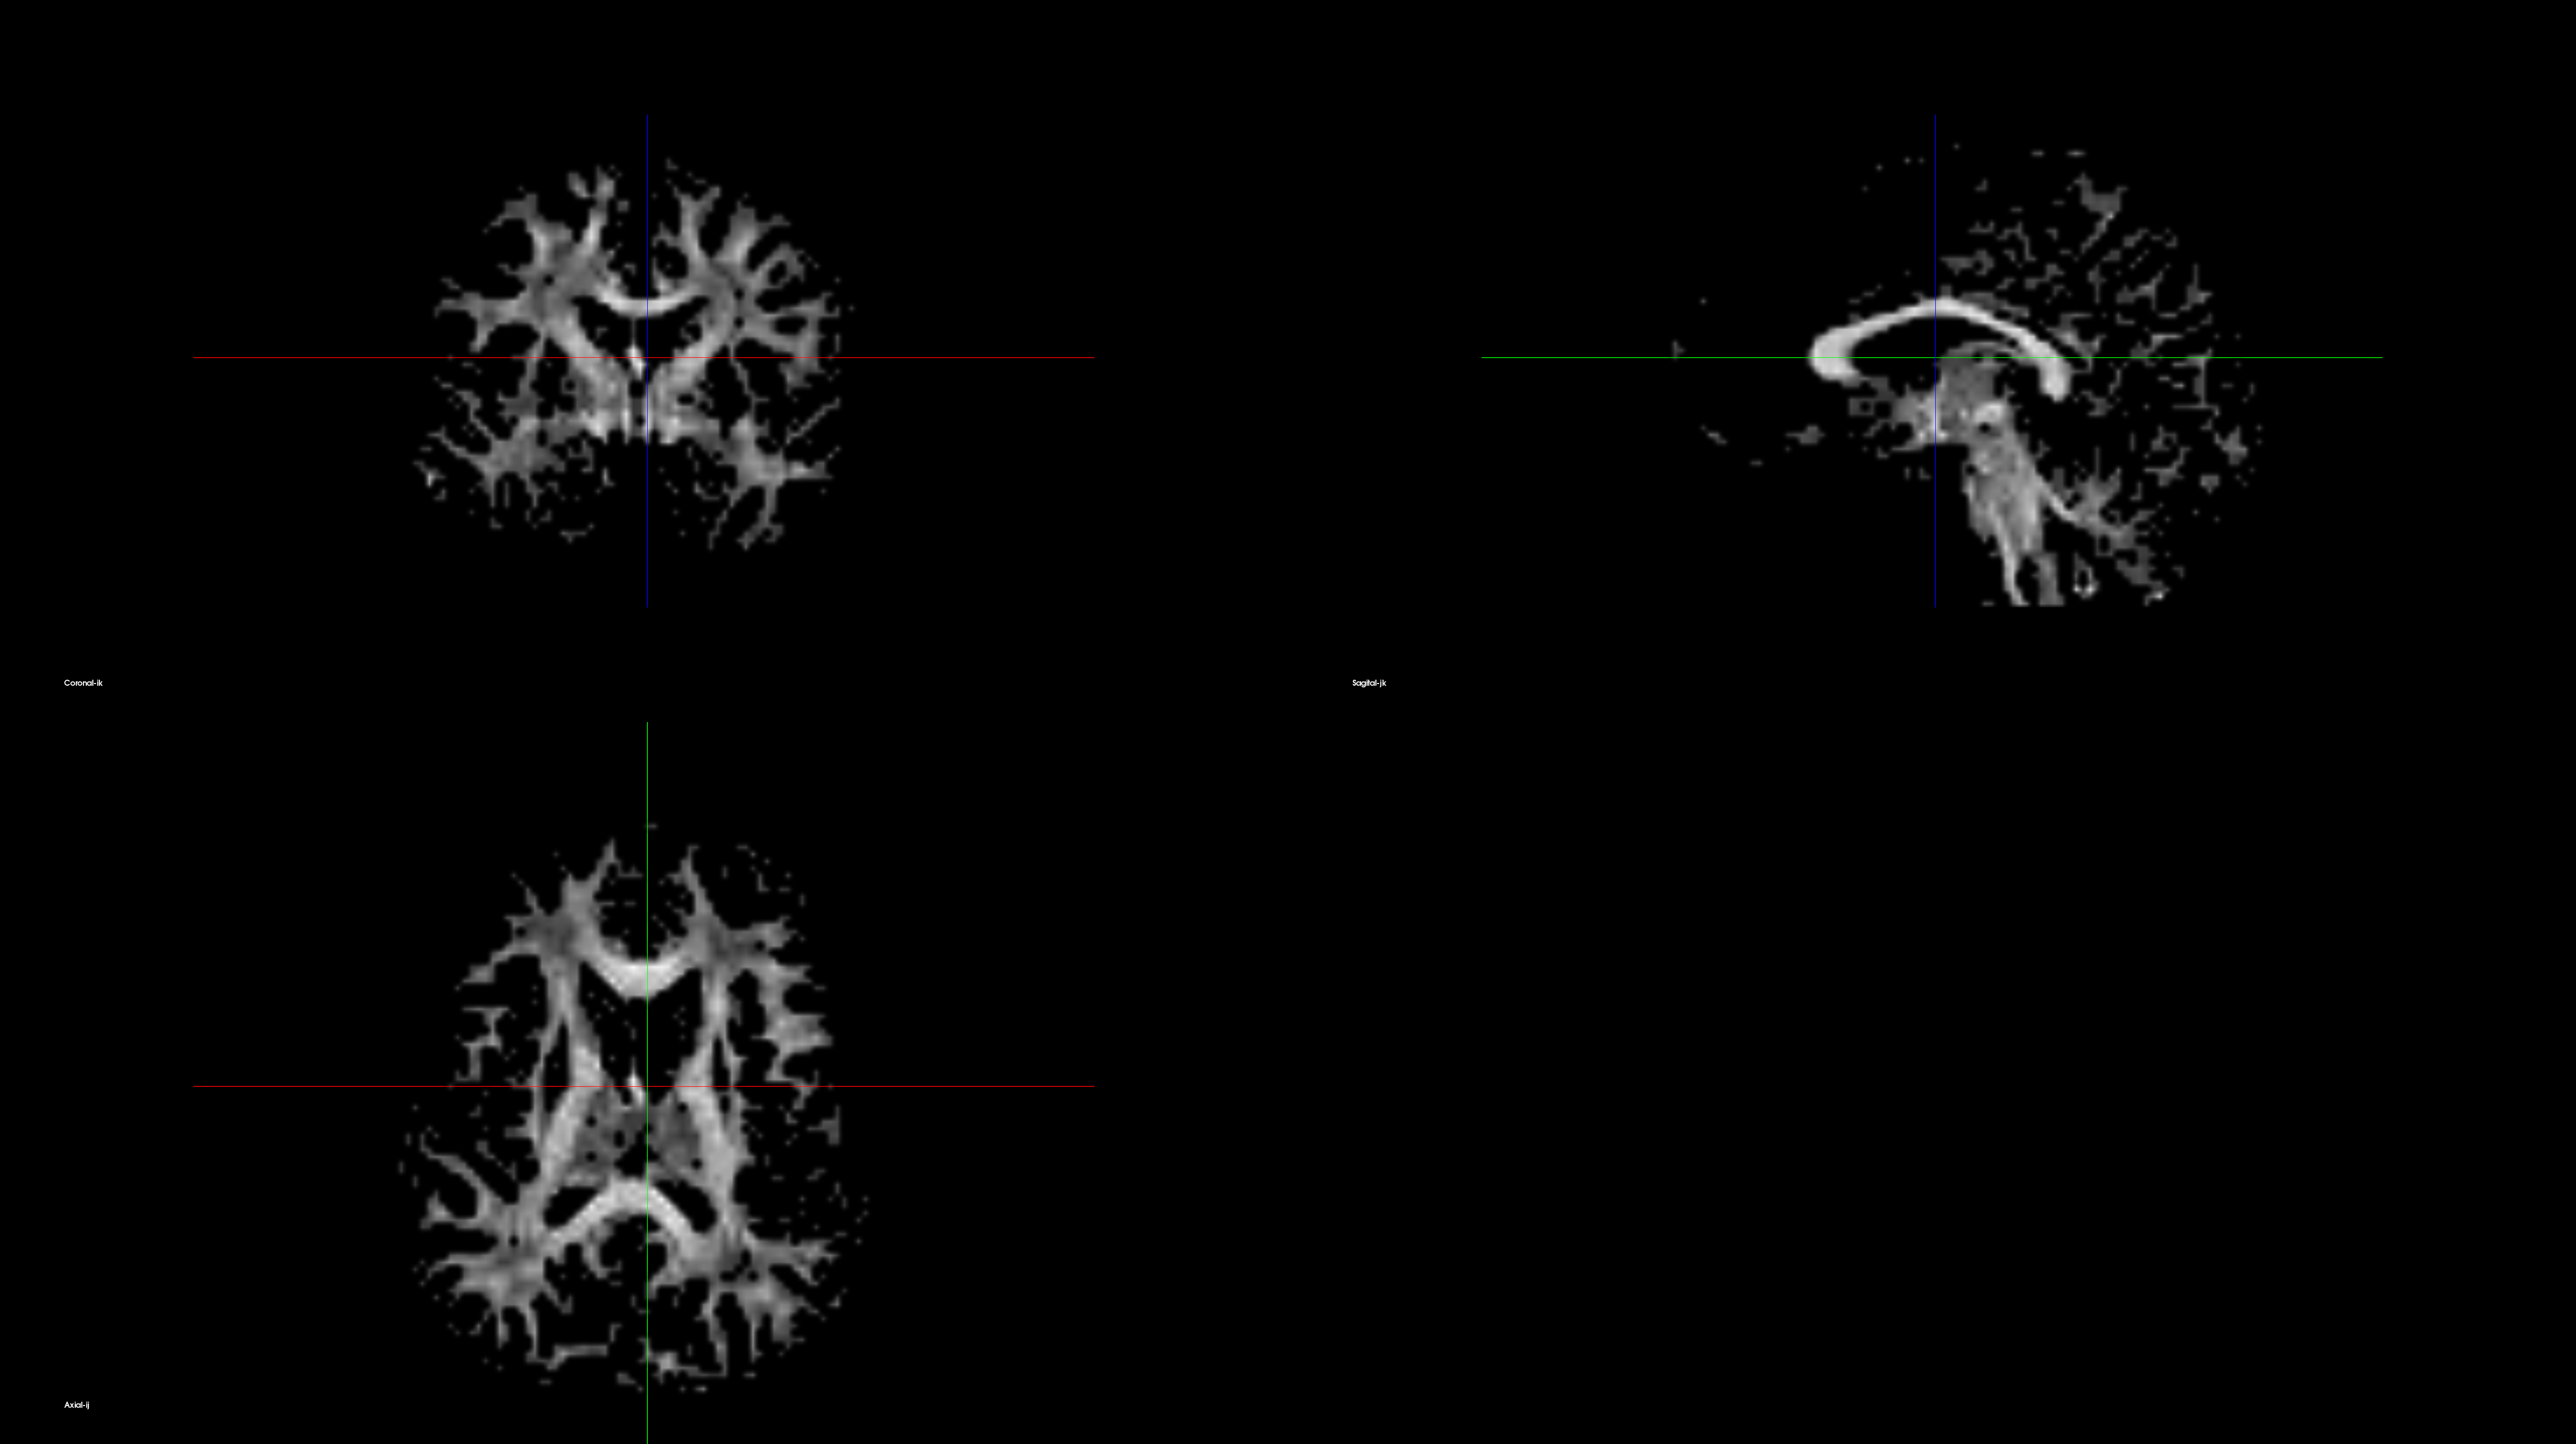
\includegraphics[width=1\linewidth]{img/my_fa_threshold.png}
      \caption{FA mask that I've generated applied to the loaded tensor on BIS.}
      \label{subfig:my_fa_threshold}
    \end{subfigure}

    \caption{Comparison between FA threshold from BIS and the one I've implemented. Both screenshots were taken from the 3-slice view mode at the position (64, 64, 35). As you can see, the results are identical.}
    \label{fig:bis-my-comparison}
  \end{figure}

  This kind of comparison exemplified by the figure above (\ref{fig:bis-my-comparison}) were really important to identify mistakes that I've made through the development like not considering the affine transformation from the original files. So, for that case, I was generating the correct mask, but it was not with the same rotations, scales and translations as the original tensor leading to different visual results.

  \section{Statistics}
  The following statistics refer to the high resolution dataset. First I'll present the statistics for the dataset with voxels with FA values under 0.2 which was the base for the clustering which I'll present just after.

    \subsection{FA threshold}\label{subsec:fa-threshold}
    After the threshold filter there were 168085 voxels left in the dataset. The time taken to generate the mask was 0m44.868s\footnote{Sequential time: 0m59.247s} and the statistics calculation took 10m41.506s\footnote{Sequential time: 10m49.423s}.

    \begin{tabular}{| c | c | c | c | c | c |}
      \hline
        & \textbf{MD} & \textbf{FA} & \textbf{RD} & \textbf{TV} & \textbf{TC} \\ \hline
       \textbf{Mean} & 0.0001473 & 0.3933297 & 0.0001154 & 0.0000000 & 0.0000009 \\ \hline
       \textbf{Standard Deviation} & 0.000053 & 0.1512194 & 0.0000468 & 0.0000000 & 0.0000005 \\ \hline 
    \end{tabular}

    \subsection{Clustering}\label{subsec:clustering}
    In order to get closer to identify a pattern to apply the clustering for each tensor metric and then look at their mean and standard deviation.

    Beyond the results, following I'll also mention the processing time taken to produce those results. For this I've used a Intel Core i7 with 4 physical cores at 2.3 GHz.

    The applied clustering algorithm was DBSCAN with 1 one voxel neighbourhood length and one point was not considered noise if it had at least 26 neighbours.

    Generally about all the clustering methods we can see from the distribution of cluster sizes (e.g. \ref{subfig:fa_hist_region}) we can see lots of small clusters and just a few huge clusters (actually two) \footnote{The following statistics will show histograms for this statistic really similar to this one.}. My insight about this is that those small clusters are the interesting ones.

    Another characteristic that was noted is the total number of clusters. The FA and TC clustering yielded almost twice clusters than RD and TV.

    \newpage
    \subsubsection{FA}
    \begin{figure}[!ht]
      \centering

      \begin{subfigure}[t]{.49\textwidth}
        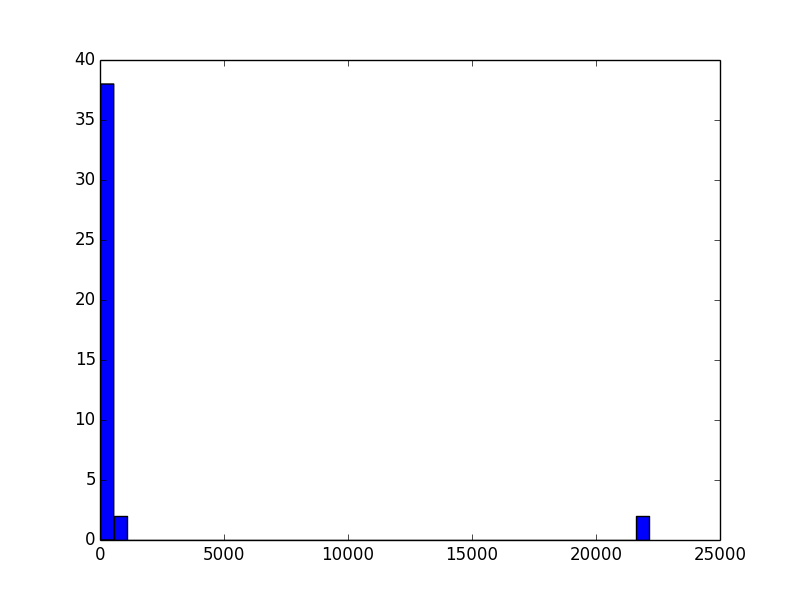
\includegraphics[width=1\linewidth]{img/histograms/fa_clustered_fa_mask_region_sizes_hist.png}
        \caption{Cluster size distribution histogram (Voxel count X Cluster count).}
        \label{subfig:fa_hist_region}
      \end{subfigure}\hfill%
      \begin{subfigure}[t]{.49\textwidth}
        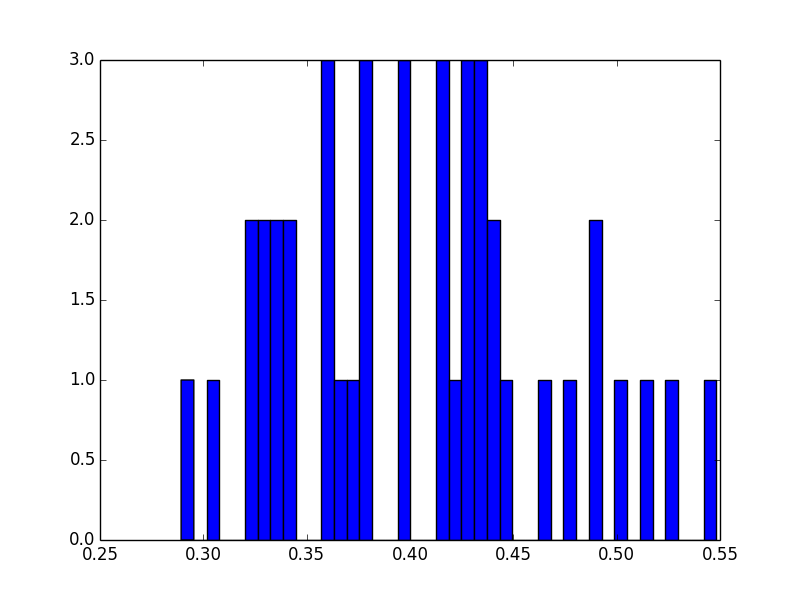
\includegraphics[width=1\linewidth]{img/histograms/fa_clustered_fa_mask_fa_means_hist.png}
        \caption{Histogram for FA mean frequency (Cluster count X FA mean).}
        \label{subfig:fa_hist_fa}
      \end{subfigure}\hfill\\
      \begin{subfigure}[t]{.49\textwidth}
        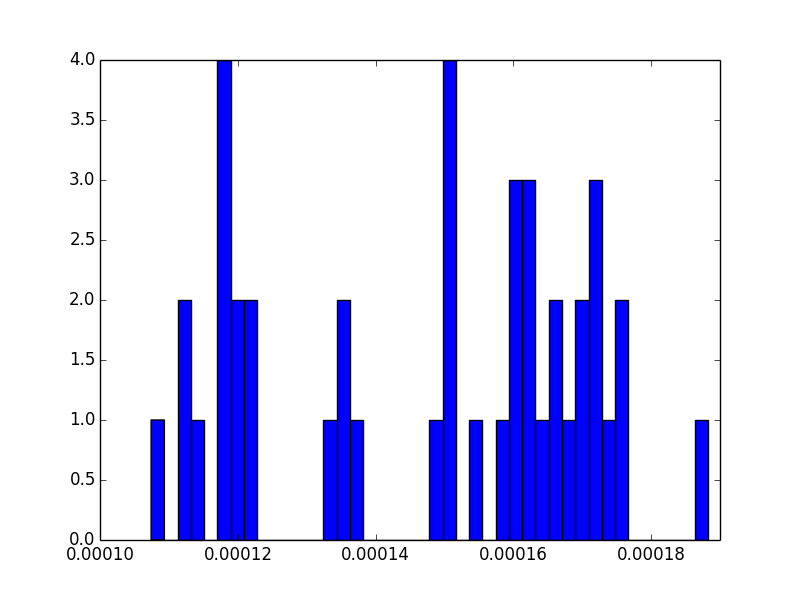
\includegraphics[width=1\linewidth]{img/histograms/fa_clustered_fa_mask_md_means_hist.png}
        \caption{Histogram for MD mean frequency (Cluster count X MD mean).}
        \label{subfig:fa_hist_md}
      \end{subfigure}\hfill%
      \begin{subfigure}[t]{.49\textwidth}
        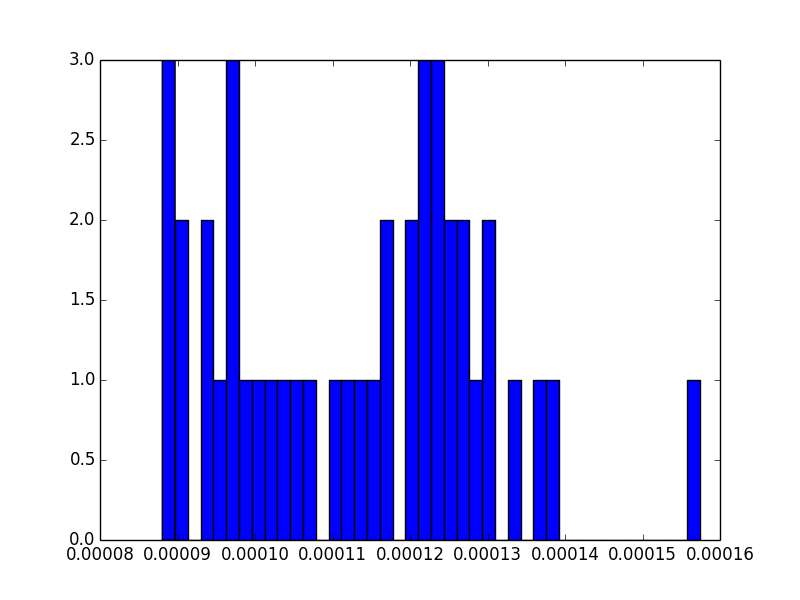
\includegraphics[width=1\linewidth]{img/histograms/fa_clustered_fa_mask_rd_means_hist.png}
        \caption{Histogram for RD mean frequency (Cluster count X RD mean).}
        \label{subfig:fa_hist_rd}
      \end{subfigure}\hfill\\
      \begin{subfigure}[t]{.49\textwidth}
        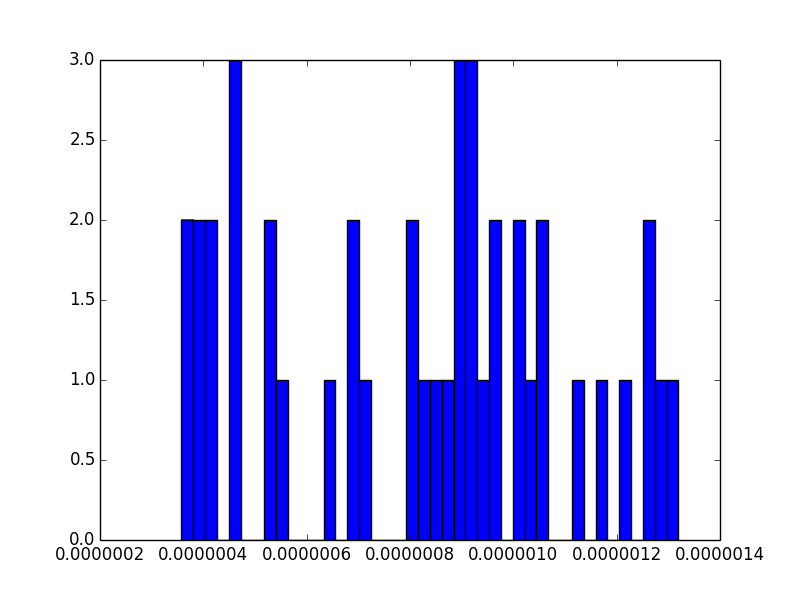
\includegraphics[width=1\linewidth]{img/histograms/fa_clustered_fa_mask_tc_means_hist.png}
        \caption{Histogram for TC mean frequency (Cluster count X TC mean).}
        \label{subfig:fa_hist_tc}
      \end{subfigure}\hfill%
      \begin{subfigure}[t]{.49\textwidth}
        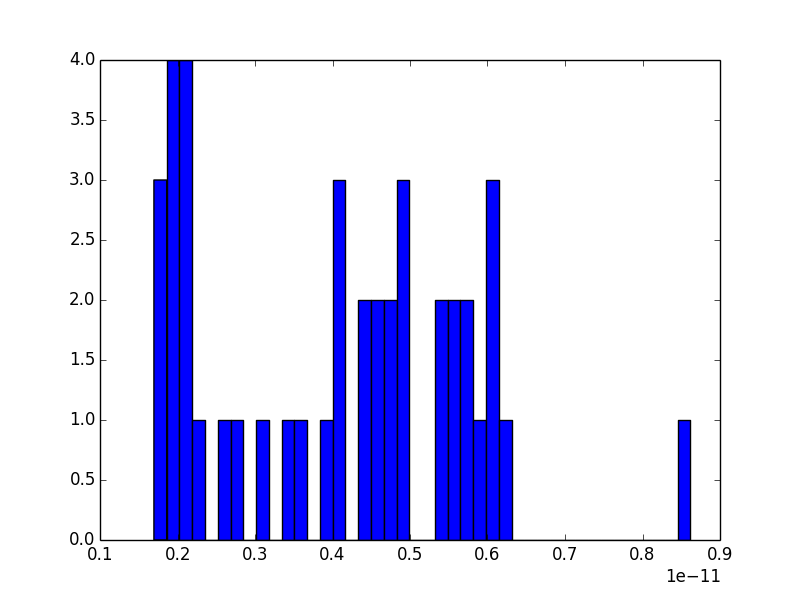
\includegraphics[width=1\linewidth]{img/histograms/fa_clustered_fa_mask_tv_means_hist.png}
        \caption{Histogram for TV mean frequency (Cluster count X TV mean).}
        \label{subfig:fa_hist_tv}
      \end{subfigure}\hfill

      \caption{Histograms for statistics distribution when clustered by FA values.}
      \label{fig:fa-histograms}
    \end{figure}

    This type of clusterization grouped voxels with FA values which don't differ no more then 0.15 (standard deviation from the entire region \ref{subsec:fa-threshold}) taking 19m32.754s\footnote{Sequential time: 13m24.782s} to get computed and another 3m18.221s\footnote{Sequential time: 3m18.922s} to generate the statistics.

    \newpage
    \subsubsection{RD}
    \begin{figure}[!ht]
      \centering

      \begin{subfigure}[t]{.49\textwidth}
        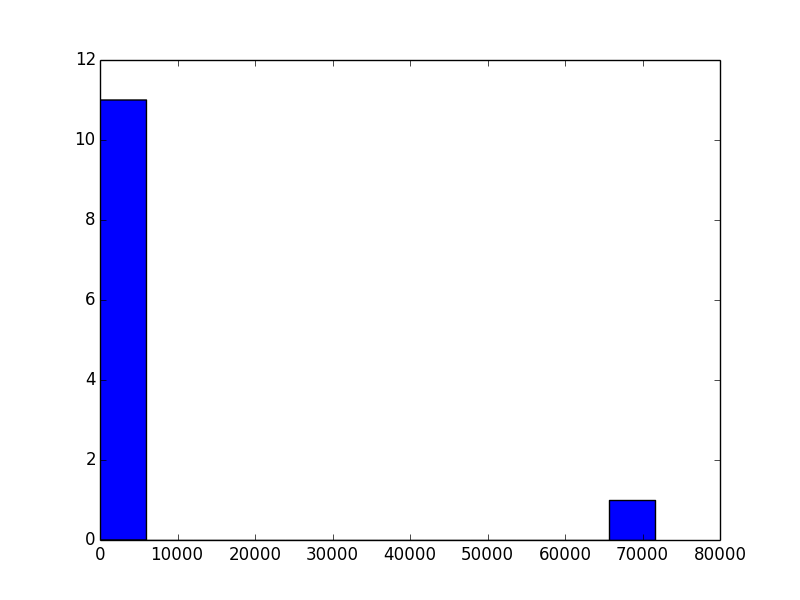
\includegraphics[width=1\linewidth]{img/histograms/rd_clustered_fa_mask_region_sizes_hist.png}
        \caption{Cluster size distribution histogram (Voxel count X Cluster count).}
        \label{subfig:fa_hist_region}
      \end{subfigure}\hfill%
      \begin{subfigure}[t]{.49\textwidth}
        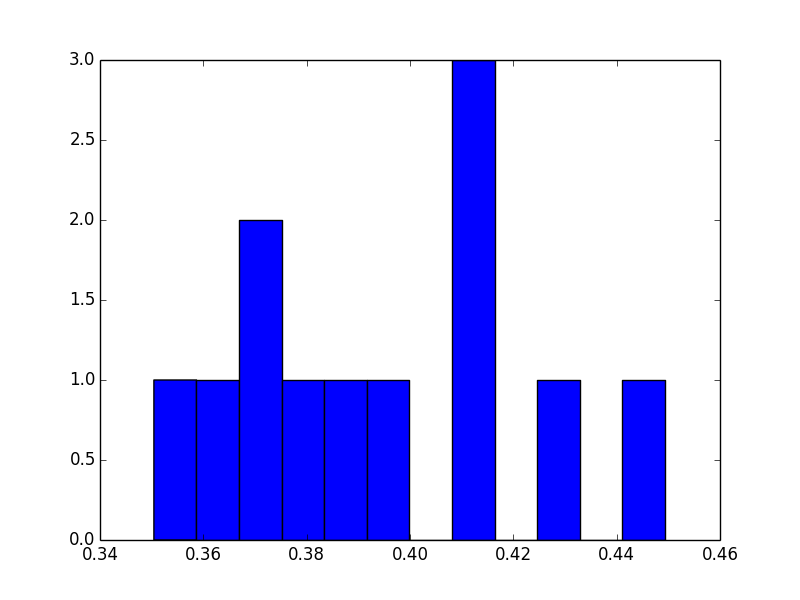
\includegraphics[width=1\linewidth]{img/histograms/rd_clustered_fa_mask_fa_means_hist.png}
        \caption{Histogram for FA mean frequency (Cluster count X FA mean).}
        \label{subfig:fa_hist_fa}
      \end{subfigure}\hfill\\
      \begin{subfigure}[t]{.49\textwidth}
        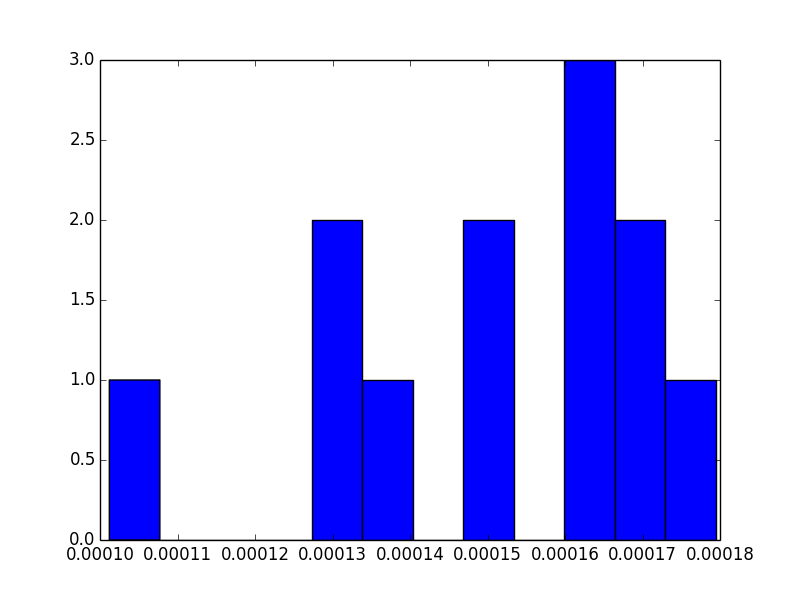
\includegraphics[width=1\linewidth]{img/histograms/rd_clustered_fa_mask_md_means_hist.png}
        \caption{Histogram for MD mean frequency (Cluster count X MD mean).}
        \label{subfig:fa_hist_md}
      \end{subfigure}\hfill%
      \begin{subfigure}[t]{.49\textwidth}
        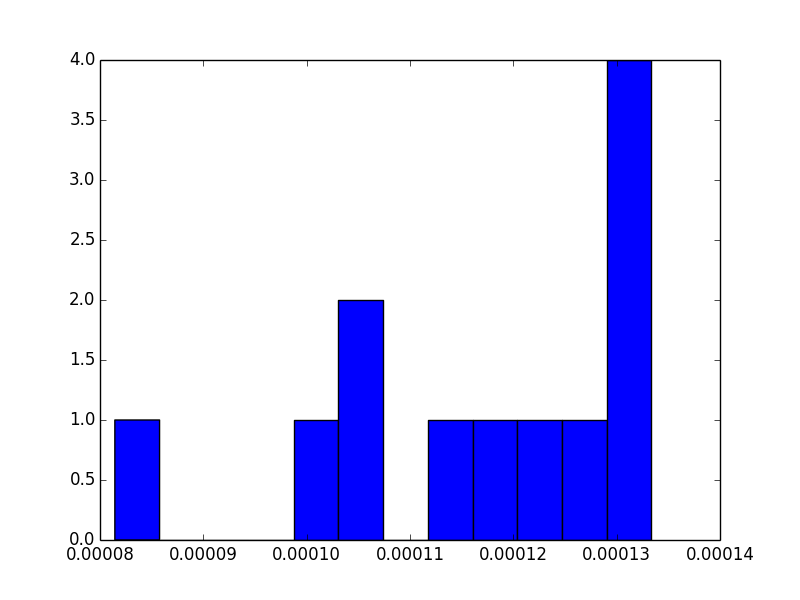
\includegraphics[width=1\linewidth]{img/histograms/rd_clustered_fa_mask_rd_means_hist.png}
        \caption{Histogram for RD mean frequency (Cluster count X RD mean).}
        \label{subfig:fa_hist_rd}
      \end{subfigure}\hfill\\
      \begin{subfigure}[t]{.49\textwidth}
        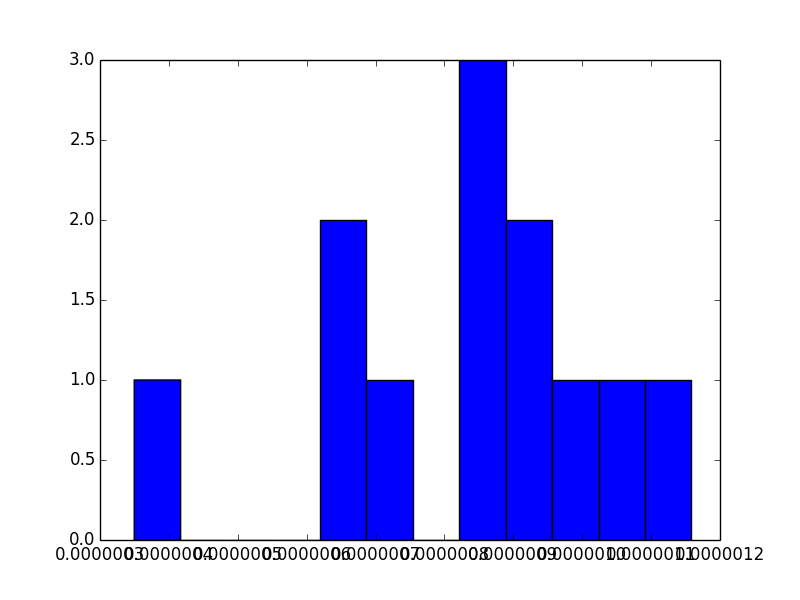
\includegraphics[width=1\linewidth]{img/histograms/rd_clustered_fa_mask_tc_means_hist.png}
        \caption{Histogram for TC mean frequency (Cluster count X TC mean).}
        \label{subfig:fa_hist_tc}
      \end{subfigure}\hfill%
      \begin{subfigure}[t]{.49\textwidth}
        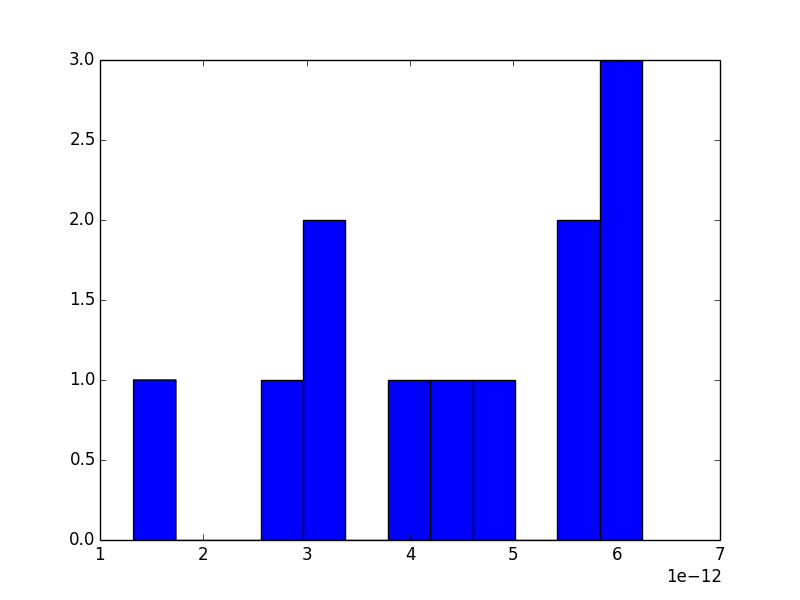
\includegraphics[width=1\linewidth]{img/histograms/rd_clustered_fa_mask_tv_means_hist.png}
        \caption{Histogram for TV mean frequency (Cluster count X TV mean).}
        \label{subfig:fa_hist_tv}
      \end{subfigure}\hfill

      \caption{Histograms for statistics distribution when clustered by RD values.}
      \label{fig:fa-histograms}
    \end{figure}

    This type of clusterization grouped voxels with RD values which don't differ no more then 0.00005 (standard deviation from the entire region \ref{subsec:fa-threshold}) taking 17m21.273s\footnote{Sequential time: 89m29.007s} to get computed and another 5m0.552s\footnote{Sequential time: 6m12.551s} to generate the statistics.

    \newpage
    \subsubsection{TC}
    \begin{figure}[!ht]
      \centering

      \begin{subfigure}[t]{.49\textwidth}
        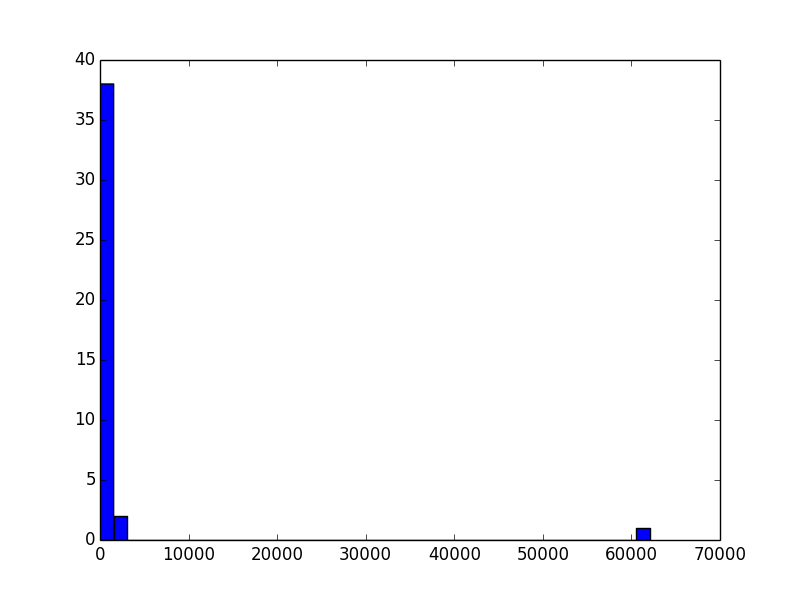
\includegraphics[width=1\linewidth]{img/histograms/tc_clustered_fa_mask_region_sizes_hist.png}
        \caption{Cluster size distribution histogram (Voxel count X Cluster count).}
        \label{subfig:fa_hist_region}
      \end{subfigure}\hfill%
      \begin{subfigure}[t]{.49\textwidth}
        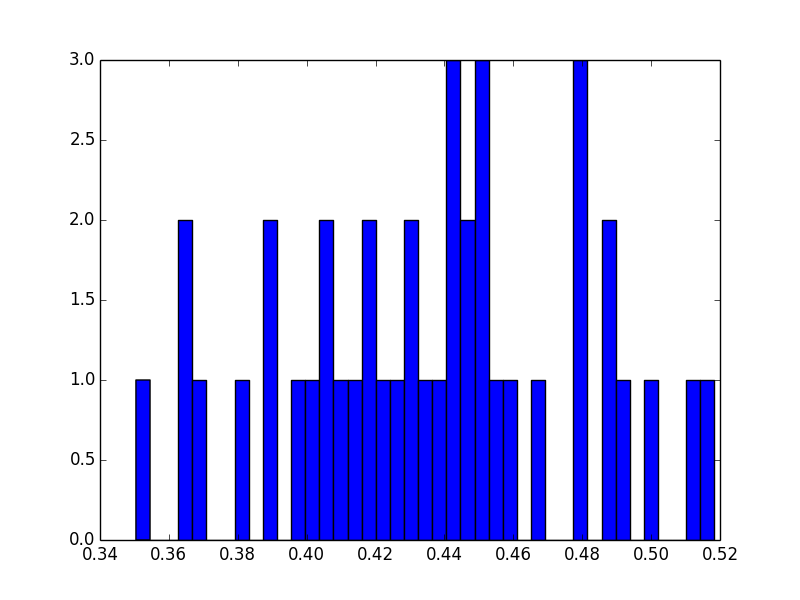
\includegraphics[width=1\linewidth]{img/histograms/tc_clustered_fa_mask_fa_means_hist.png}
        \caption{Histogram for FA mean frequency (Cluster count X FA mean).}
        \label{subfig:fa_hist_fa}
      \end{subfigure}\hfill\\
      \begin{subfigure}[t]{.49\textwidth}
        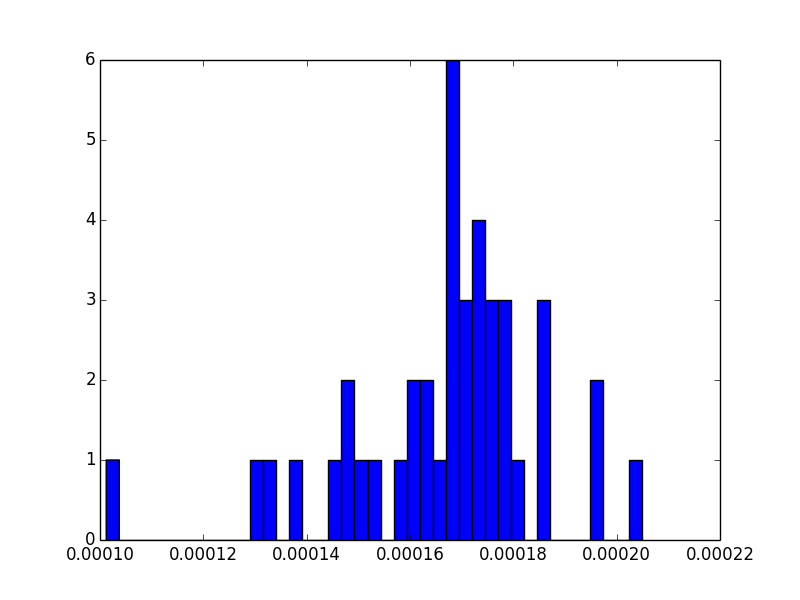
\includegraphics[width=1\linewidth]{img/histograms/tc_clustered_fa_mask_md_means_hist.png}
        \caption{Histogram for MD mean frequency (Cluster count X MD mean).}
        \label{subfig:fa_hist_md}
      \end{subfigure}\hfill%
      \begin{subfigure}[t]{.49\textwidth}
        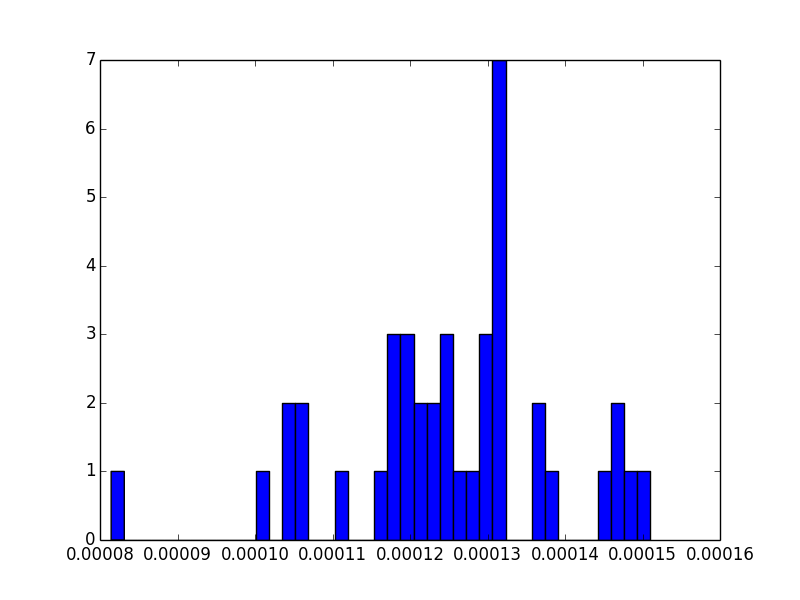
\includegraphics[width=1\linewidth]{img/histograms/tc_clustered_fa_mask_rd_means_hist.png}
        \caption{Histogram for RD mean frequency (Cluster count X RD mean).}
        \label{subfig:fa_hist_rd}
      \end{subfigure}\hfill\\
      \begin{subfigure}[t]{.49\textwidth}
        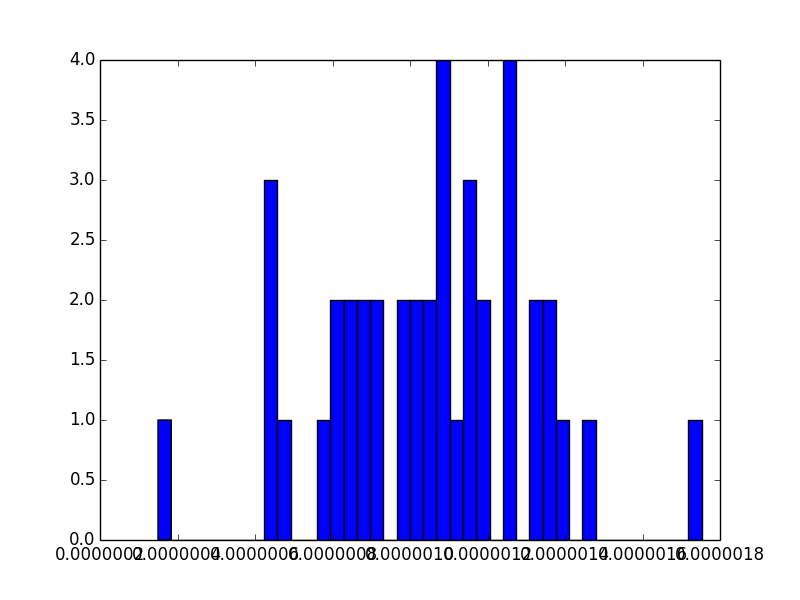
\includegraphics[width=1\linewidth]{img/histograms/tc_clustered_fa_mask_tc_means_hist.png}
        \caption{Histogram for TC mean frequency (Cluster count X TC mean).}
        \label{subfig:fa_hist_tc}
      \end{subfigure}\hfill%
      \begin{subfigure}[t]{.49\textwidth}
        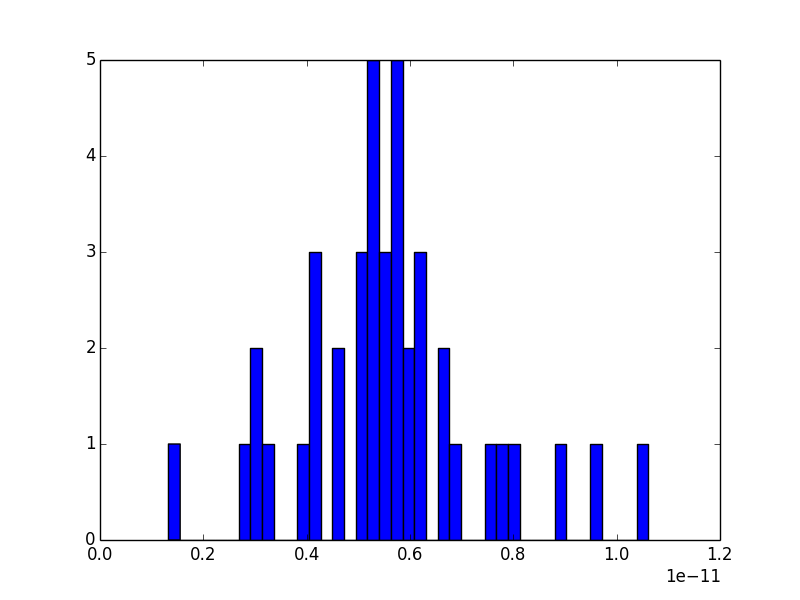
\includegraphics[width=1\linewidth]{img/histograms/tc_clustered_fa_mask_tv_means_hist.png}
        \caption{Histogram for TV mean frequency (Cluster count X TV mean).}
        \label{subfig:fa_hist_tv}
      \end{subfigure}\hfill

      \caption{Histograms for statistics distribution when clustered by TC values.}
      \label{fig:fa-histograms}
    \end{figure}

    This type of clusterization grouped voxels with FA values which don't differ no more then 0.0000005 (standard deviation from the entire region \ref{subsec:fa-threshold}) taking 62m17.542s\footnote{Sequential time: 76m56.386s} to get computed and another 4m34.027s\footnote{Sequential time: 4m11.423s} to generate the statistics.

    \newpage
    \subsubsection{TV}
    \begin{figure}[!ht]
      \centering

      \begin{subfigure}[t]{.49\textwidth}
        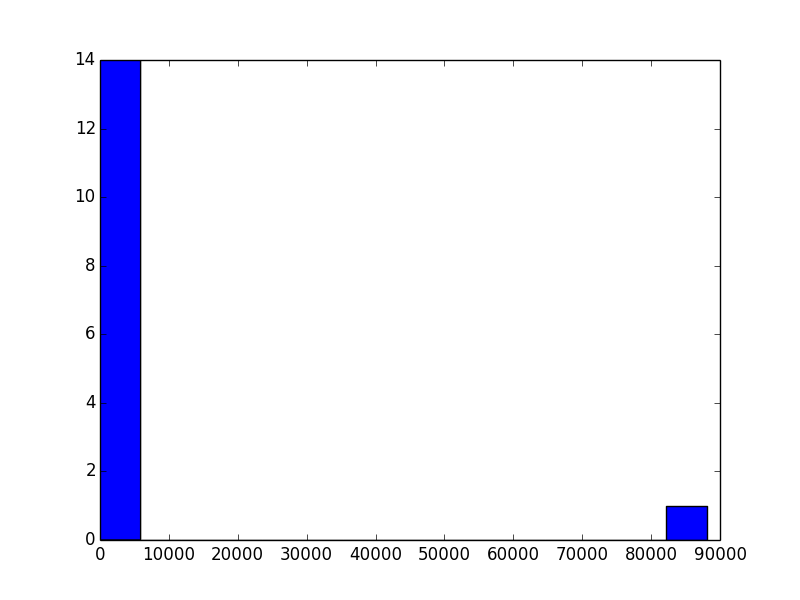
\includegraphics[width=1\linewidth]{img/histograms/tv_clustered_fa_mask_region_sizes_hist.png}
        \caption{Cluster size distribution histogram (Voxel count X Cluster count).}
        \label{subfig:fa_hist_region}
      \end{subfigure}\hfill%
      \begin{subfigure}[t]{.49\textwidth}
        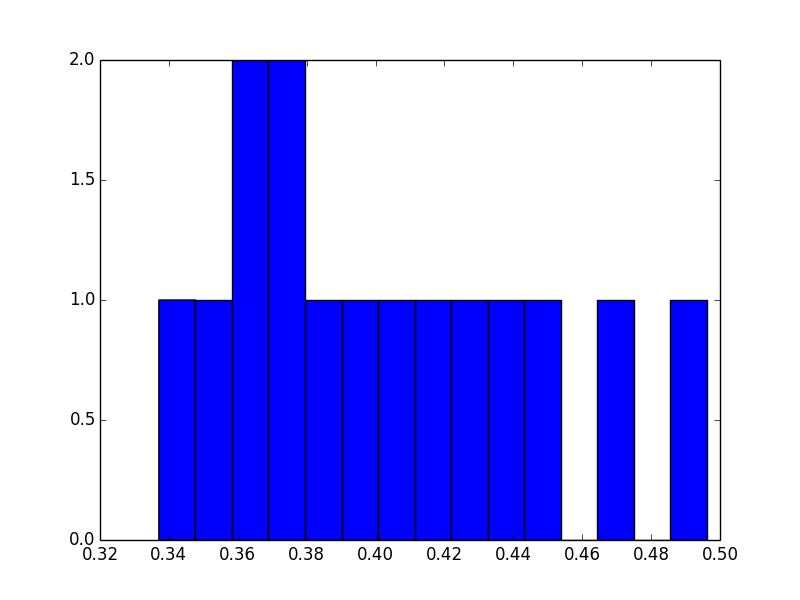
\includegraphics[width=1\linewidth]{img/histograms/tv_clustered_fa_mask_fa_means_hist.png}
        \caption{Histogram for FA mean frequency (Cluster count X FA mean).}
        \label{subfig:fa_hist_fa}
      \end{subfigure}\hfill\\
      \begin{subfigure}[t]{.49\textwidth}
        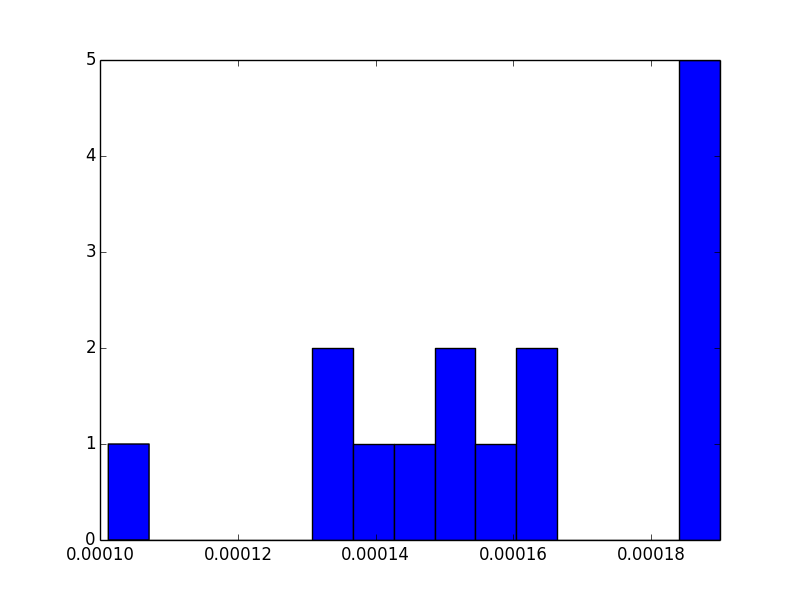
\includegraphics[width=1\linewidth]{img/histograms/tv_clustered_fa_mask_md_means_hist.png}
        \caption{Histogram for MD mean frequency (Cluster count X MD mean).}
        \label{subfig:fa_hist_md}
      \end{subfigure}\hfill%
      \begin{subfigure}[t]{.49\textwidth}
        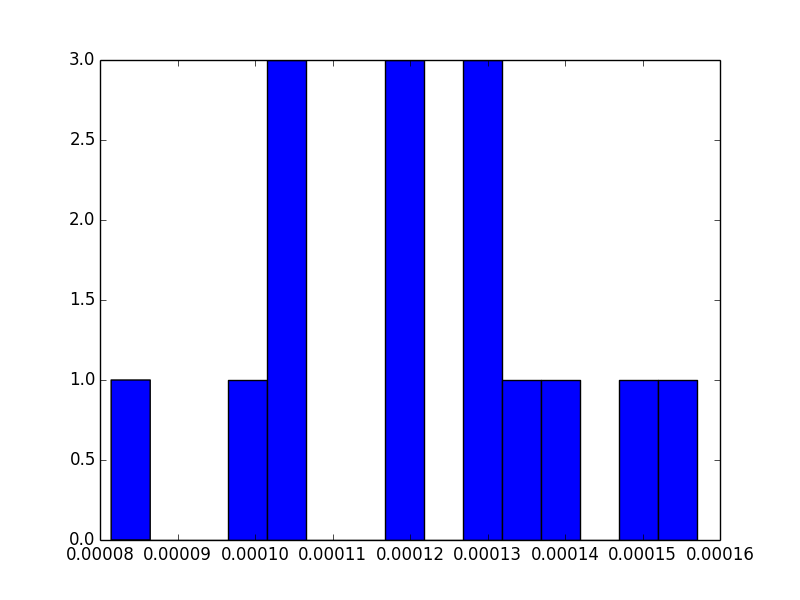
\includegraphics[width=1\linewidth]{img/histograms/tv_clustered_fa_mask_rd_means_hist.png}
        \caption{Histogram for RD mean frequency (Cluster count X RD mean).}
        \label{subfig:fa_hist_rd}
      \end{subfigure}\hfill\\
      \begin{subfigure}[t]{.49\textwidth}
        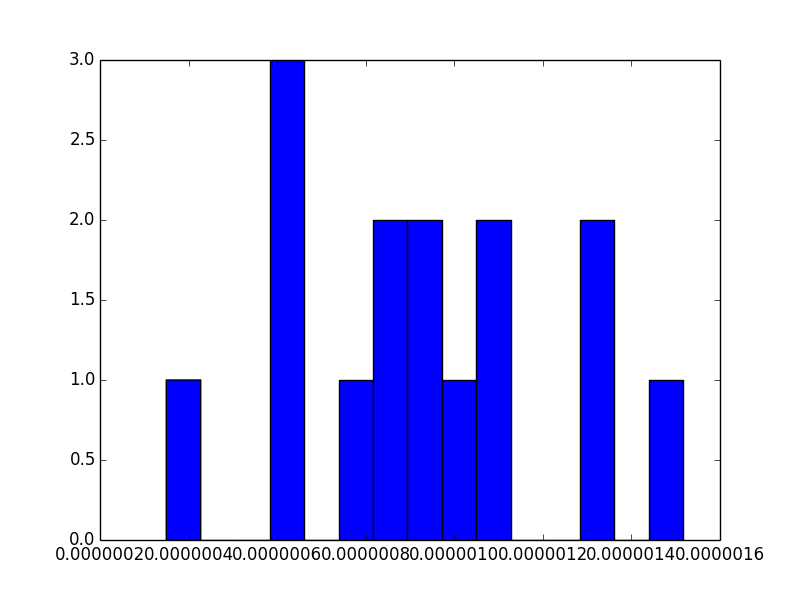
\includegraphics[width=1\linewidth]{img/histograms/tv_clustered_fa_mask_tc_means_hist.png}
        \caption{Histogram for TC mean frequency (Cluster count X TC mean).}
        \label{subfig:fa_hist_tc}
      \end{subfigure}\hfill%
      \begin{subfigure}[t]{.49\textwidth}
        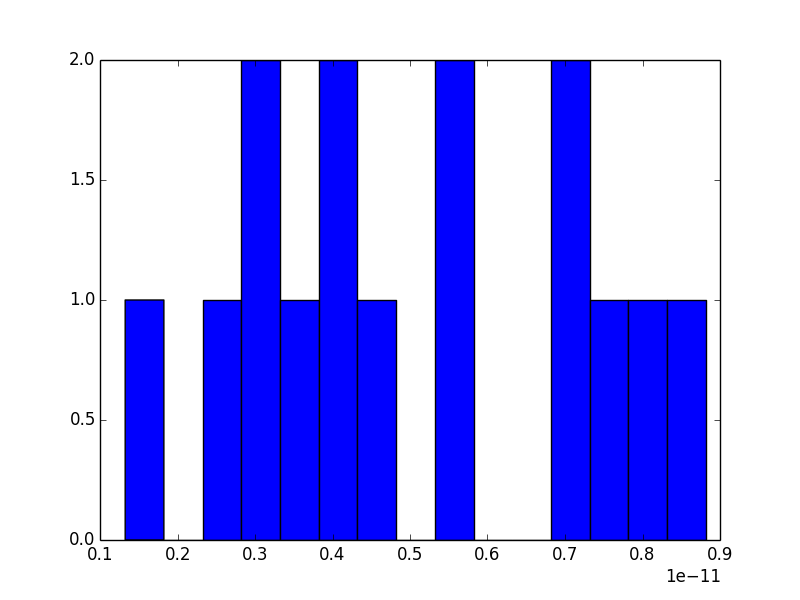
\includegraphics[width=1\linewidth]{img/histograms/tv_clustered_fa_mask_tv_means_hist.png}
        \caption{Histogram for TV mean frequency (Cluster count X TV mean).}
        \label{subfig:fa_hist_tv}
      \end{subfigure}\hfill

      \caption{Histograms for statistics distribution when clustered by TV values.}
      \label{fig:fa-histograms}
    \end{figure}

    This type of clusterization grouped voxels with FA values which don't differ no more then 0.00000001 taking 17m29.473s\footnote{Sequential time: 137m11.281s} to get computed and another 6m24.052s\footnote{Sequential time: 5m38.443s} to generate the statistics.

\chapter{Conclusion}
Most of the statistics, except for the cluster size, doesn't look really meaningful alone. In order to make any affirmations more experiments are necessary involving more datasets so maybe the other statistics may show some kind of pattern that we can explore for the task of identifying fiber crossing regions.

The hypothesis mentioned on \ref{subsec:clustering} that raises the question about the size of crossing regions may be answered with more anatomical knowledge about known crossing regions in the brain or with a well mapped phantom dataset.

So with this knowledge I may be able to compare and see if any of these clusterization methods are getting any closer to map crossing regions and, if so, which of them is the most promising one.

\end{document}